
\section{Idade do pai ou responsável ao nascimento}\label{var_interesse}

Nossa variável de interesse, relativa à idade do pai, apresenta pouca documentação acerca de sua implementação e manutenção no Sinasc. A DNV passou por alguns processos de atualização. \citeonline{jorge2007quality} afirmam que no primeiro modelo de DNV estavam presentes campos para registros das seguintes informações: cartório de registro e o local de ocorrência do nascimento, informações sobre o recém-nascido (data do nascimento, sexo, peso ao nascer, índice de Apgar) e sobre a gravidez (duração da gestação, tipo de gravidez e tipo de parto), características da mãe do nascido vivo (nome, idade, grau de instrução, município de residência e filhos tidos) e nome do pai. Porém, em janeiro de 1996, já passa a circular um novo modelo de DNV no país, no qual o campo para registro do nome do pai foi retirado \cite{jorge2007quality}.

\citeonline{mello1993avaliaccao} já apontavam (quando o sistema de informação sobre nascimentos era ainda operado pelo Instituto Brasileiro de Geografia e Estatística, com base nas informações do Registro Civil) sobre comportamento atípico para a variável nome do pai, em relação às demais onde, segundo eles, “a ausência de informação, neste caso, não implica, necessariamente, falha de preenchimento, podendo, também, retratar o desejo de não identificar o pai.” \cite[p.21]{mello1993avaliaccao}. Relataram, ainda, que no estudo que realizam em cinco municípios de São Paulo, um dos municípios não possuia registro para a informação porque o único hospital da cidade\footnote{Município de Pariquera-Açu.}, à época, decidiu deliberadamente omitir o dado. Concluíram que a informação relativa ao nome do pai estava sendo pouco valorizada pelos estabelecimentos de saúde. Em trecho que exprimem sua opinião, os autores afirmam: “Essa atitude vem ao encontro de opinião dos autores que julgam ser o nome do pai uma informação de caráter jurídico e não médico, epidemiológico, ou de saúde pública e, portanto, dispensável em um documento dessa natureza.”\cite[p.21]{mello1993avaliaccao}.

Não foi possível verificar porque o campo (nome do pai) foi retirado em 1996, já no âmbito do Sinasc. Somente através do dicionário de variáveis disponível no site da Secretaria de Vigilância em Saúde e Ambiente \footnote{Fonte: \href{https://svs.aids.gov.br/daent/cgiae/sinasc/documentacao/dicionario_de_dados_SINASC_tabela_DN.pdf}{Dicionário de dados da tabela DN.}} foi possível identificar que as variáveis que registram informações sobre a paternidade do nascido vivo (a saber, nome e idade do pai) fazem parte de um conjunto de novos campos criados em 2009. 

A mudança da DNV em que é introduzida, aparentemente, pela primeira vez, o registro da idade do pai ao nascimento, foi discutida e aprovada no Comitê Técnico Assessor do SIM (Sistema de informação sobre Mortalidade) e Sinasc no período de 2007 a 2009 \cite{BRConsolidacaoSINASC2011}. O processo de implementação se deu de forma gradual, após realização de teste piloto, o novo formulário foi ajustado e impresso em 2010. O CTA decidiu por uma estratégia de não substituir abruptamente a DNV antiga pela nova versão, fazendo com que o modelo antigo e o novo circulassem simultaneamente.

Apesar da orientação de que, a partir de janeiro de 2011, fosse utilizado preferencialmente os formulários novos, naquele ano ainda houve uma proporção expressiva dos nascimentos sendo registrados no modelo antigo da DNV. Segundo relatório da Coordenação Geral de Informações e Análise Epidemiológica \cite{BRConsolidacaoSINASC2011}, a base de dados do Sinasc de 2011 é constituída de 58\% de formulários novos (com informação para idade do pai), e 42\% de formulários antigos. Por região, a participação do formulário novo variou, sendo maior no Nordeste (88\%), e menor no Sudeste (35\%). O Centro-Oeste teve, proporcionalmente, a segunda maior utilização de formulário novos (76\%), seguido pelo Norte (68\%), e pelo Sul (39\%). Devido aos campos com informações sobre a paternidade serem coletados somente a partir do novo modelo adotado em 2009, a análise terá início em 2012.

Em sua última atualização, o 8º modelo da DNV distribuído a partir de agosto de 2021, os campos para registro de informações paternas foram modificados, para se adequar a novos modelos de parentalidade e arranjos familiares\footnote{Fonte: NOTA TÉCNICA Nº 195/2021-CGIAE/DASNT/SVS/MS. Disponível em: https://dive.sc.gov.br/phocadownload/SINASC/Legisla\%C3\%A7\%C3\%A3o/NTF-n195-2021.pdf}.
O “bloco IV - Pai”, contendo o nome e idade do pai, passa a ser “Bloco IV– Responsável legal”, onde deve ser registrado o nome do(s) responsável(eis) legal(ais)\footnote{É possível registrar, inclusive, dois responsáveis legais, nesse caso, fica registrada a idade do  primeiro responsável legal inscrito.} \cite{BRmanualDNV2022}. Os campos para registro das informações paternas, desde sua implementação 2009-2010, não são de preenchimento obrigatório e não é necessário, nem suficiente, para o reconhecimento da paternidade. Ou seja, ter o nome do pai registrado na DNV não dá legitimidade legal à paternidade do nascido vivo, esse procedimento é somente realizado em cartório \cite{BRmanualDNV2011}. A não utilização dos termos “pai” e “mãe” ocorre para que seja contemplada a filiação, independentemente da identidade de gênero, como nos casos de reprodução assistida, casais transgêneros, união homoafetiva e outras situações similares. Nos campos para “Responsável legal” não têm, necessariamente, a idade do genitor do nascido vivo registrada. Porém, admite-se que o registro de nascimentos havidos por reprodução assistida ou de gestação por substituição ainda ocorram em proporção tal que não devem alterar as estimativas.

Fazendo uma avaliação da completude do preenchimento para a variável idade do pai ou responsável no Sinasc, podemos avaliar que 2012 foi o ano com menor proporção de registros ignorados. No decorrer dos anos, a completude da variável apresenta piora, chegando a mais de 60\% de dado faltante de 2018 em diante (gráfico \ref{graf:FaltanteBrasil})\footnote{Os gráficos apresentados nessa seção serão alterados para contemplar os anos de 2021 e 2022.}. Tal comportamento pode decorrer da falta de valorização destinada à variável, como ilustrado pela perspectiva de \citeonline{mello1993avaliaccao}, da percepção dessa informação como algo não associado à saúde pública ou sem valor jurídico (para a afirmação da paternidade) e, portanto, vista como não valiosa para o contexto do documento. 

\begin{grafico}
    \centering
    \caption{Percentual de dados faltantes para a idade do pai ou responsável - Brasil - 2012-2020}
    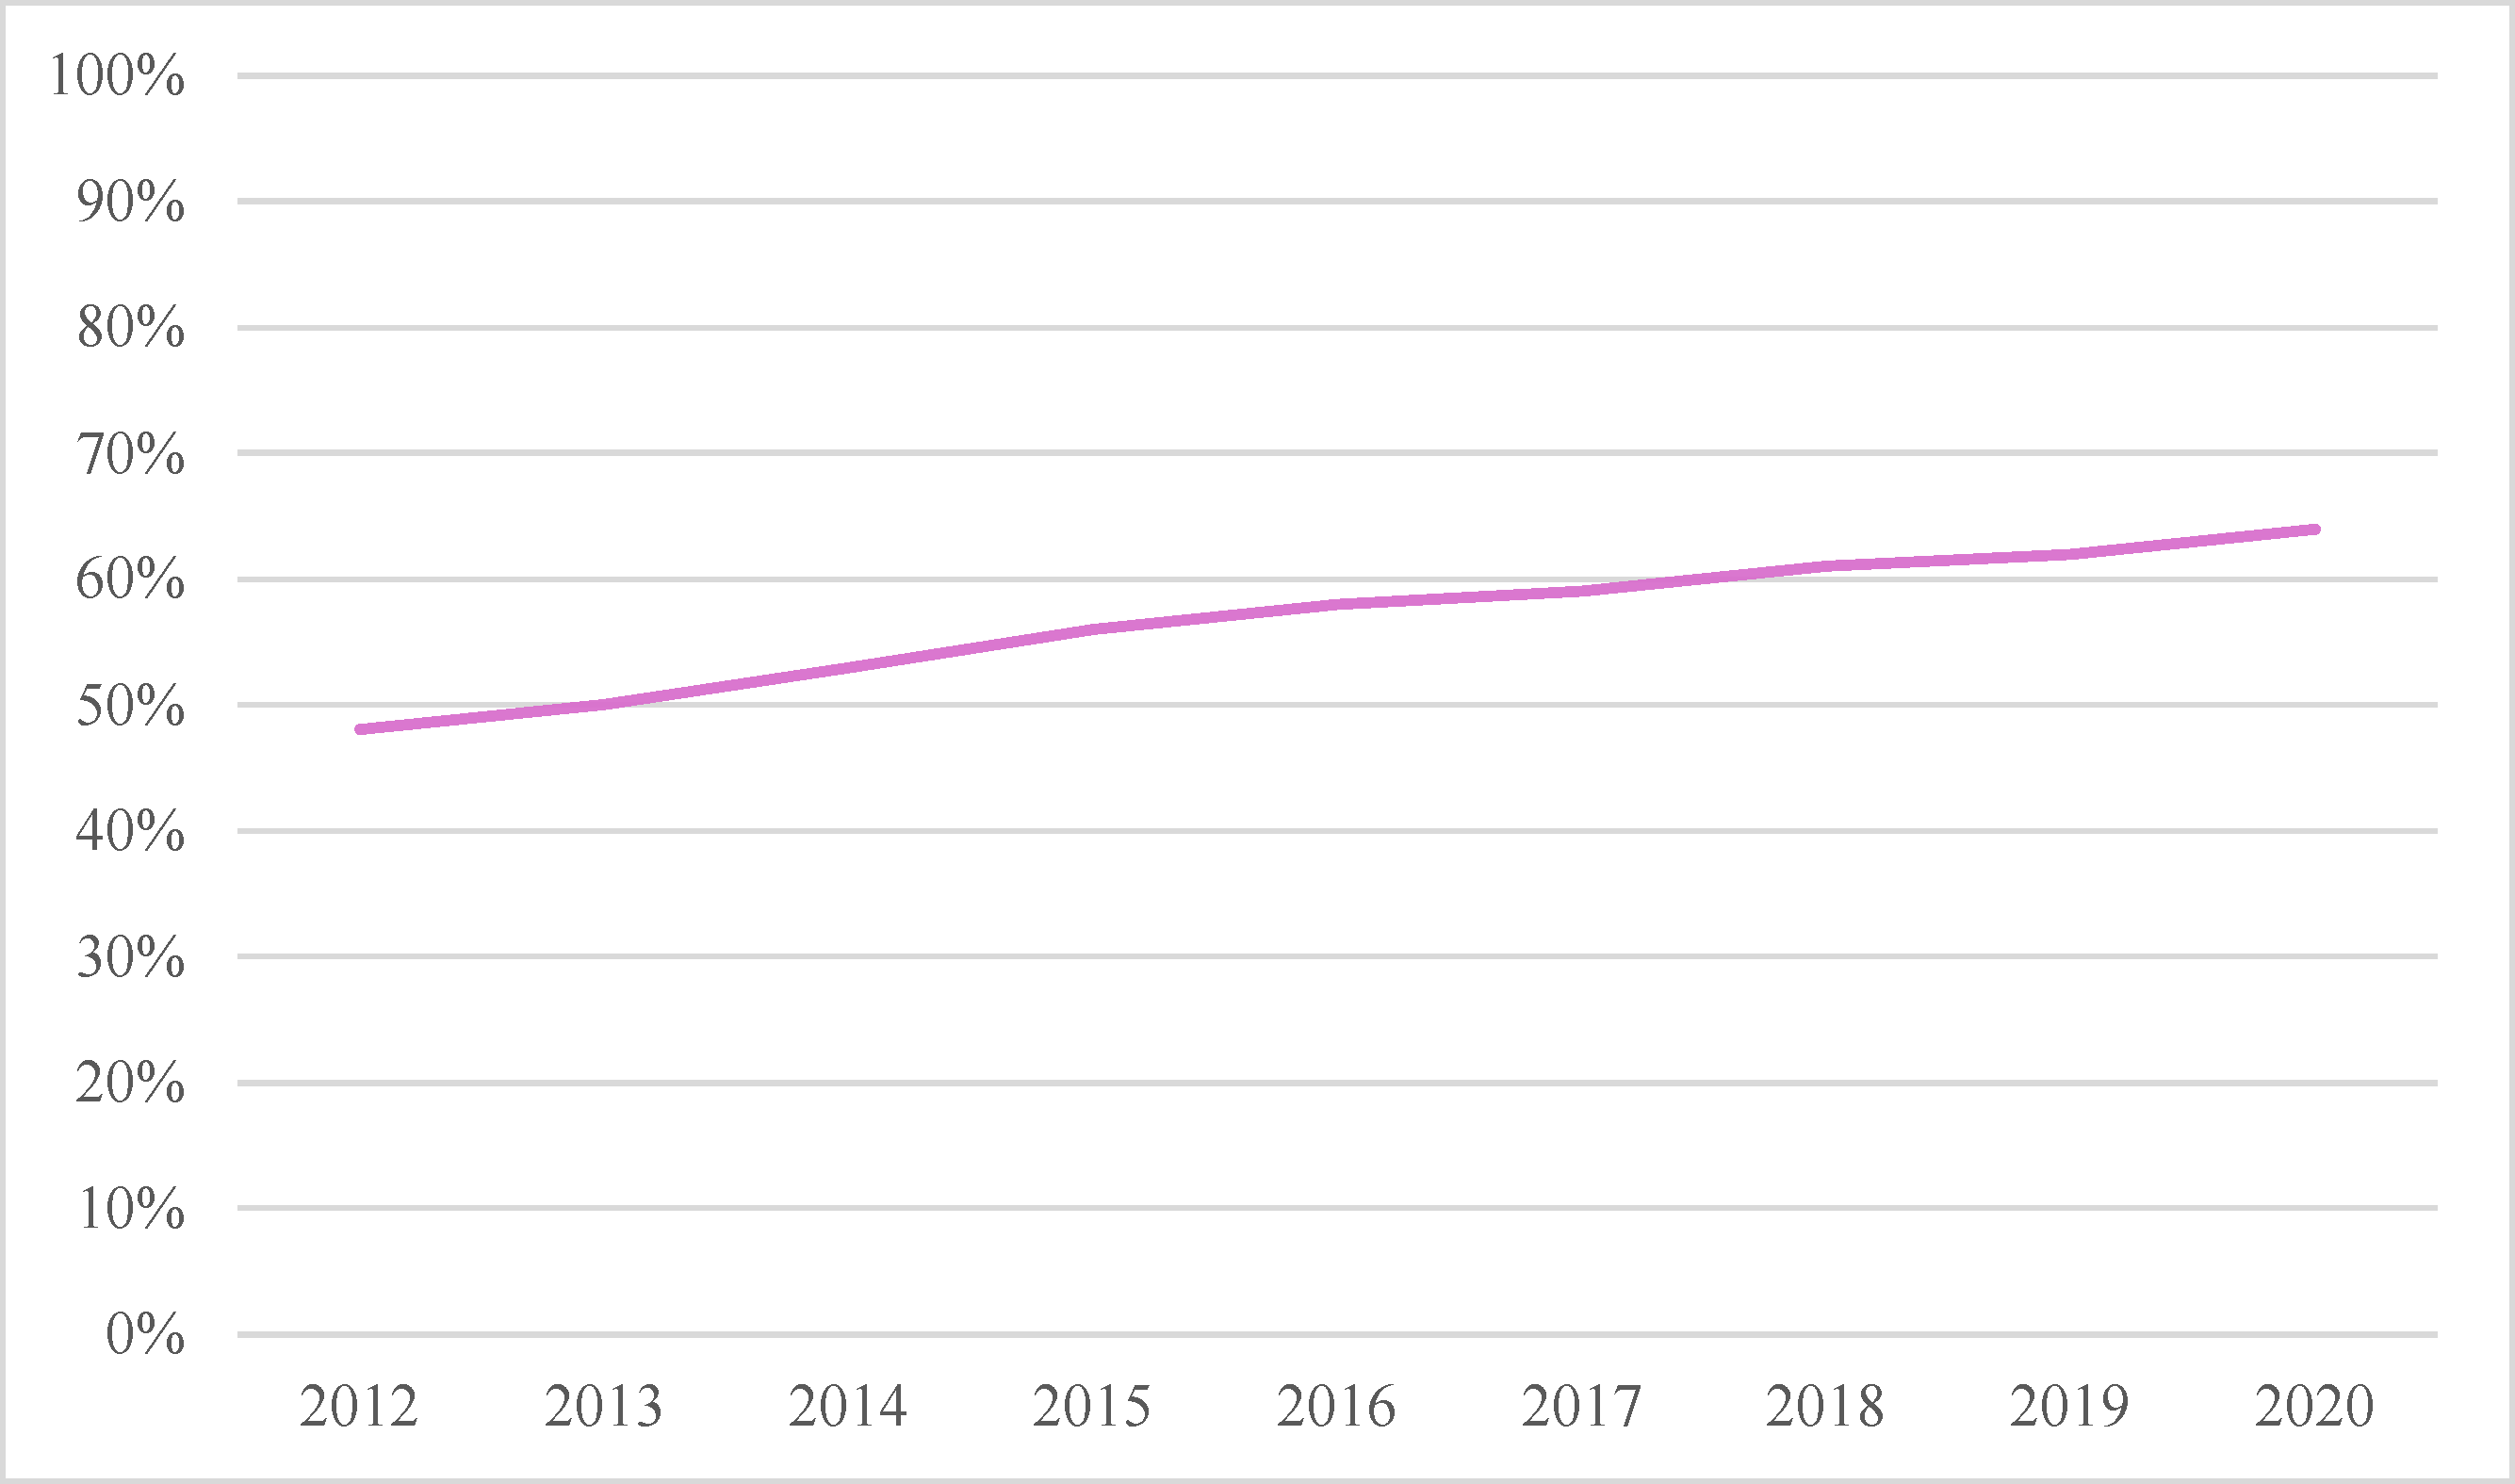
\includegraphics[width=5.0in]{imagens/Proporção de dados faltantes para idade do pai 2010-2020 nível Brasil.pdf}
    \fonte{Datasus - Sinasc}
    \label{graf:FaltanteBrasil}
\end{grafico}

A distribuição dos valores faltantes não acontece de maneira homogênea entre as regiões e UFs. Observando os gráficos \ref{graf:sudeste} ao \ref{graf:nordeste} vemos comportamentos diferentes. A região Sudeste apresenta percentuais semelhantes de valores faltantes entre as UFs, com valores concentrados entre 30\% e 40\% no início do período e entre 50\% e 60\% em 2020.

\begin{grafico}
    \centering  
    \caption{Percentual de dados faltantes para a idade do pai ou responsável - Região Sudeste - 2012-2020}
    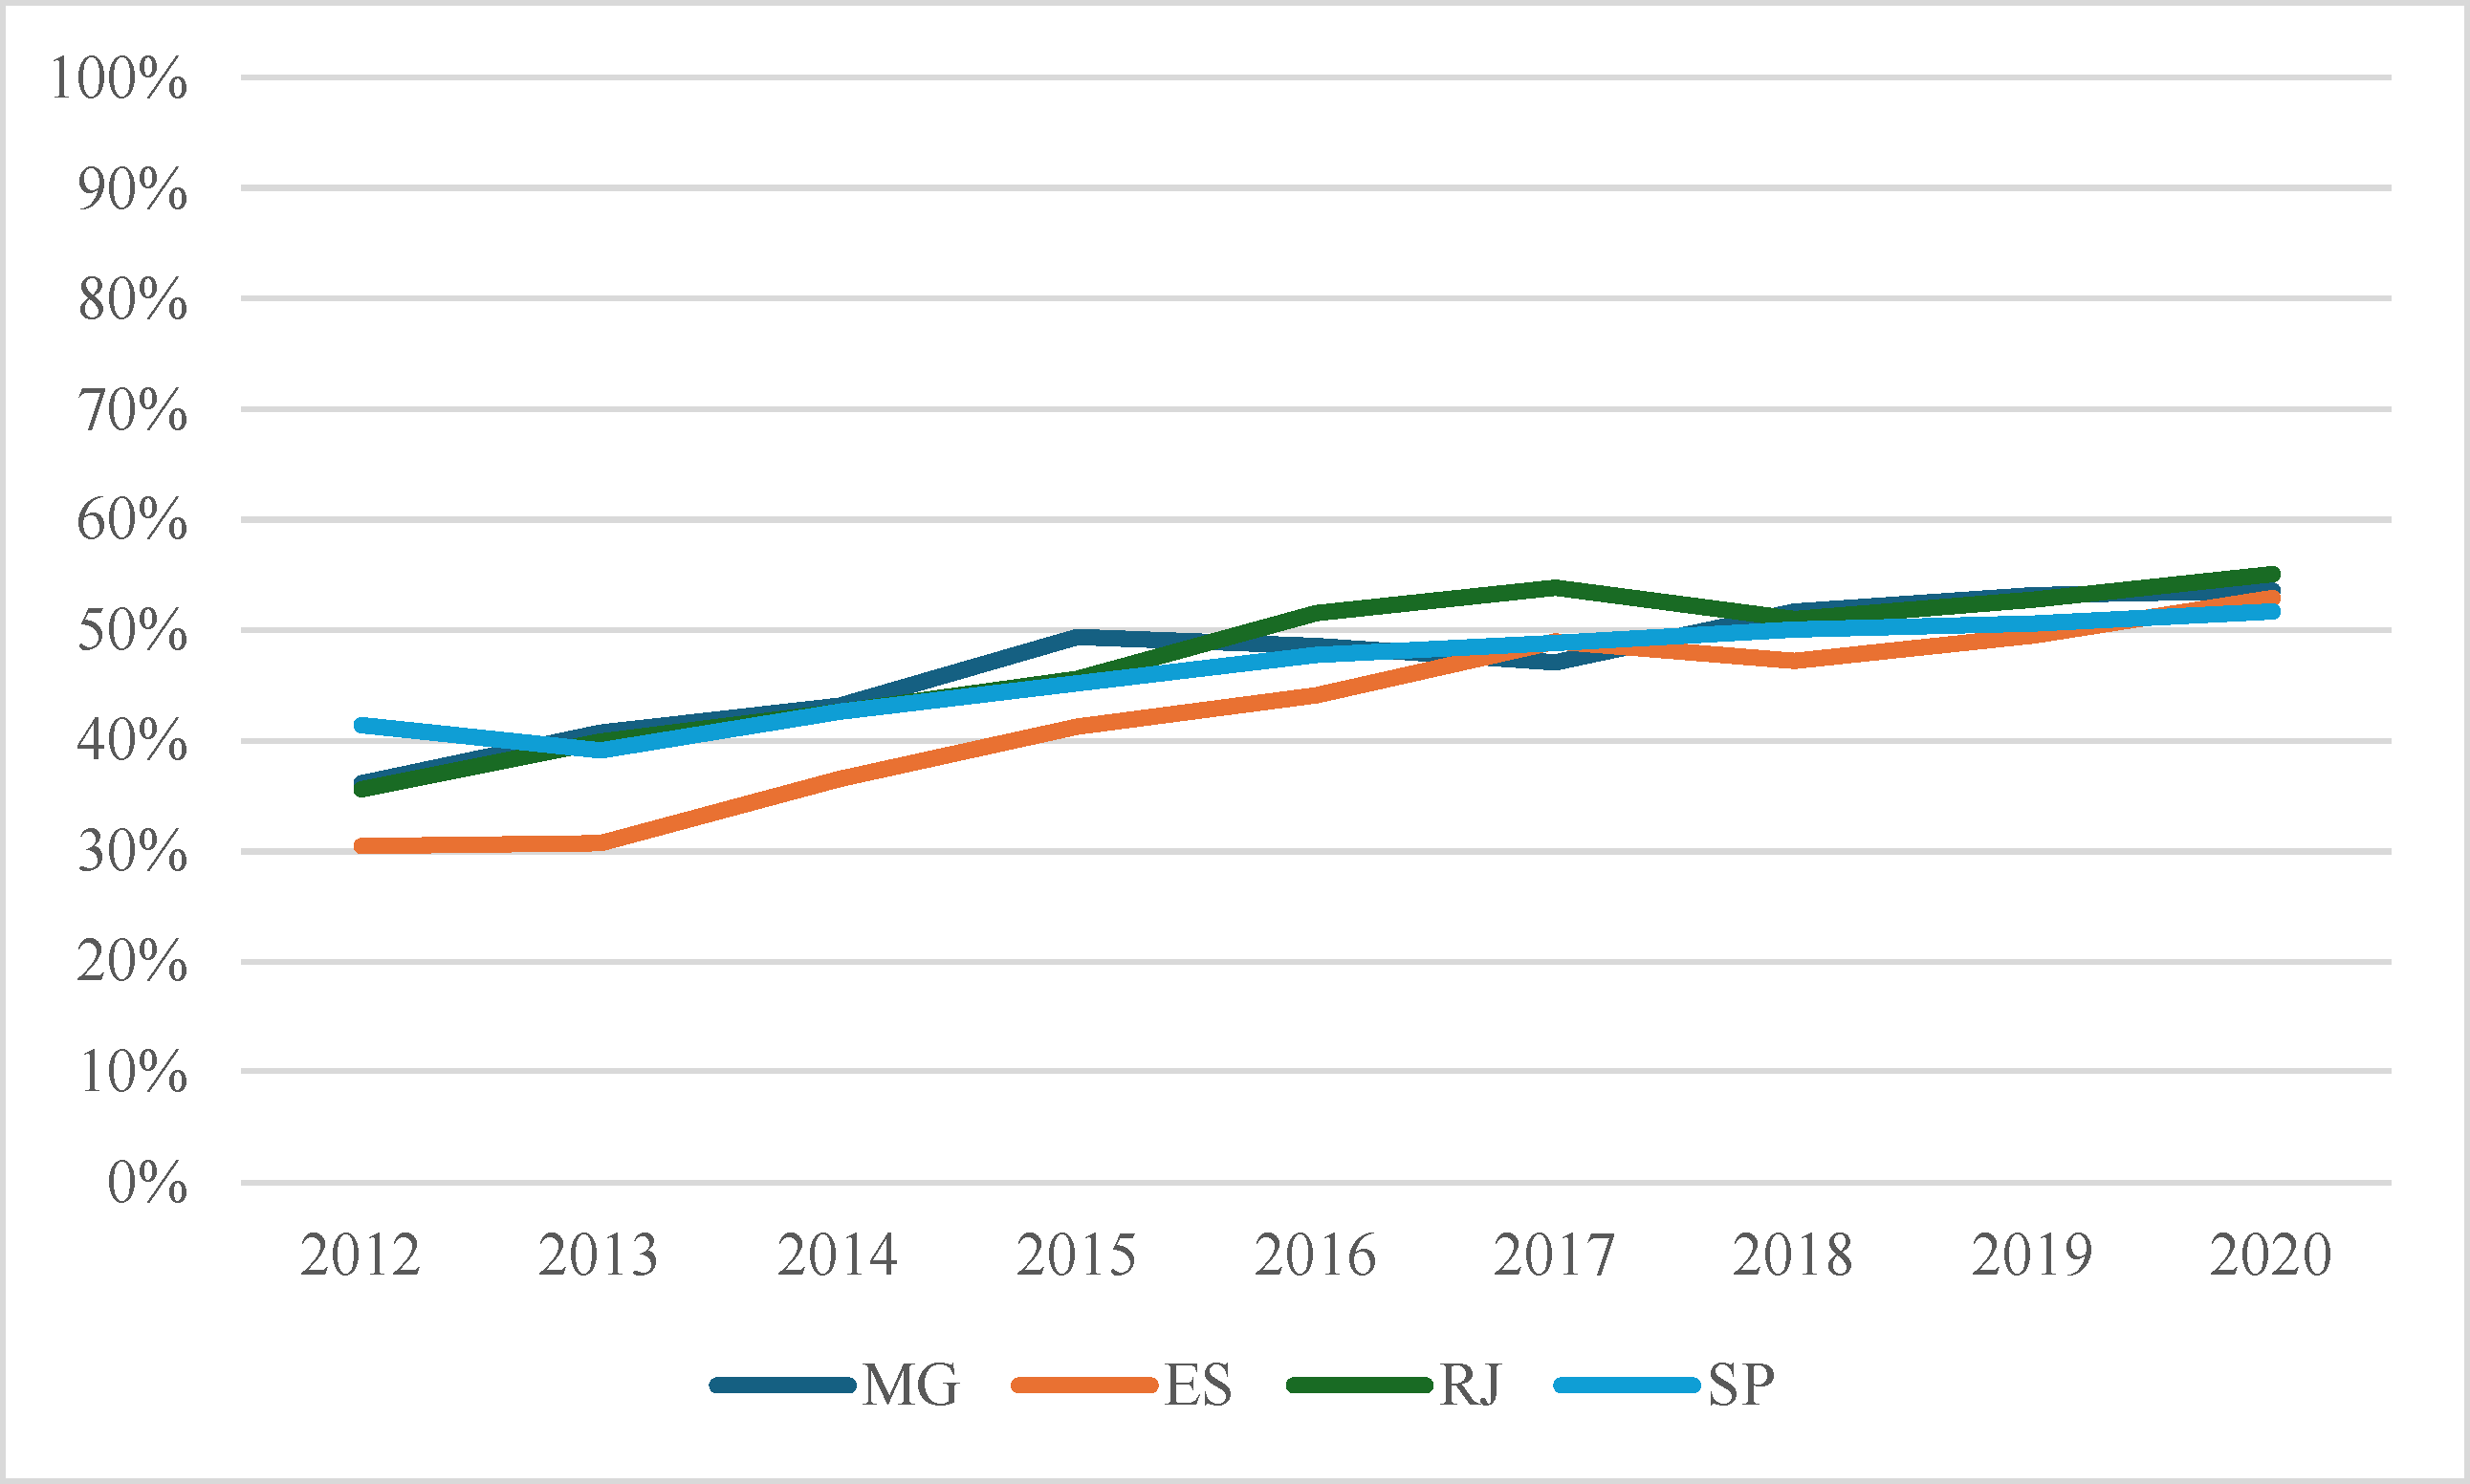
\includegraphics[width=5.0in]{imagens/faltantes-sudeste.pdf}
    \fonte{Datasus - Sinasc}
    \label{graf:sudeste}
\end{grafico}

Já os valores para o gráfico \ref{graf:sul} são mais discrepantes entre os estados, com Santa Catarina apresentando 45\% de dado faltante em 2012, enquanto Paraná o valor encontrado foi de 13\% para o mesmo ano. O Paraná foi a UF que apresentou as menores proporções de dados faltantes no período. Observa-se, porém, que o padrão de crescimento da não observação da idade do pai também ocorre no estado, alcançando o mesmo nível de dado faltante que o Rio Grande do Sul em 2020, em 33\%.

\begin{grafico}
    \centering  
    \caption{Percentual de dados faltantes para a idade do pai ou responsável - Região Sul - 2012-2020}
        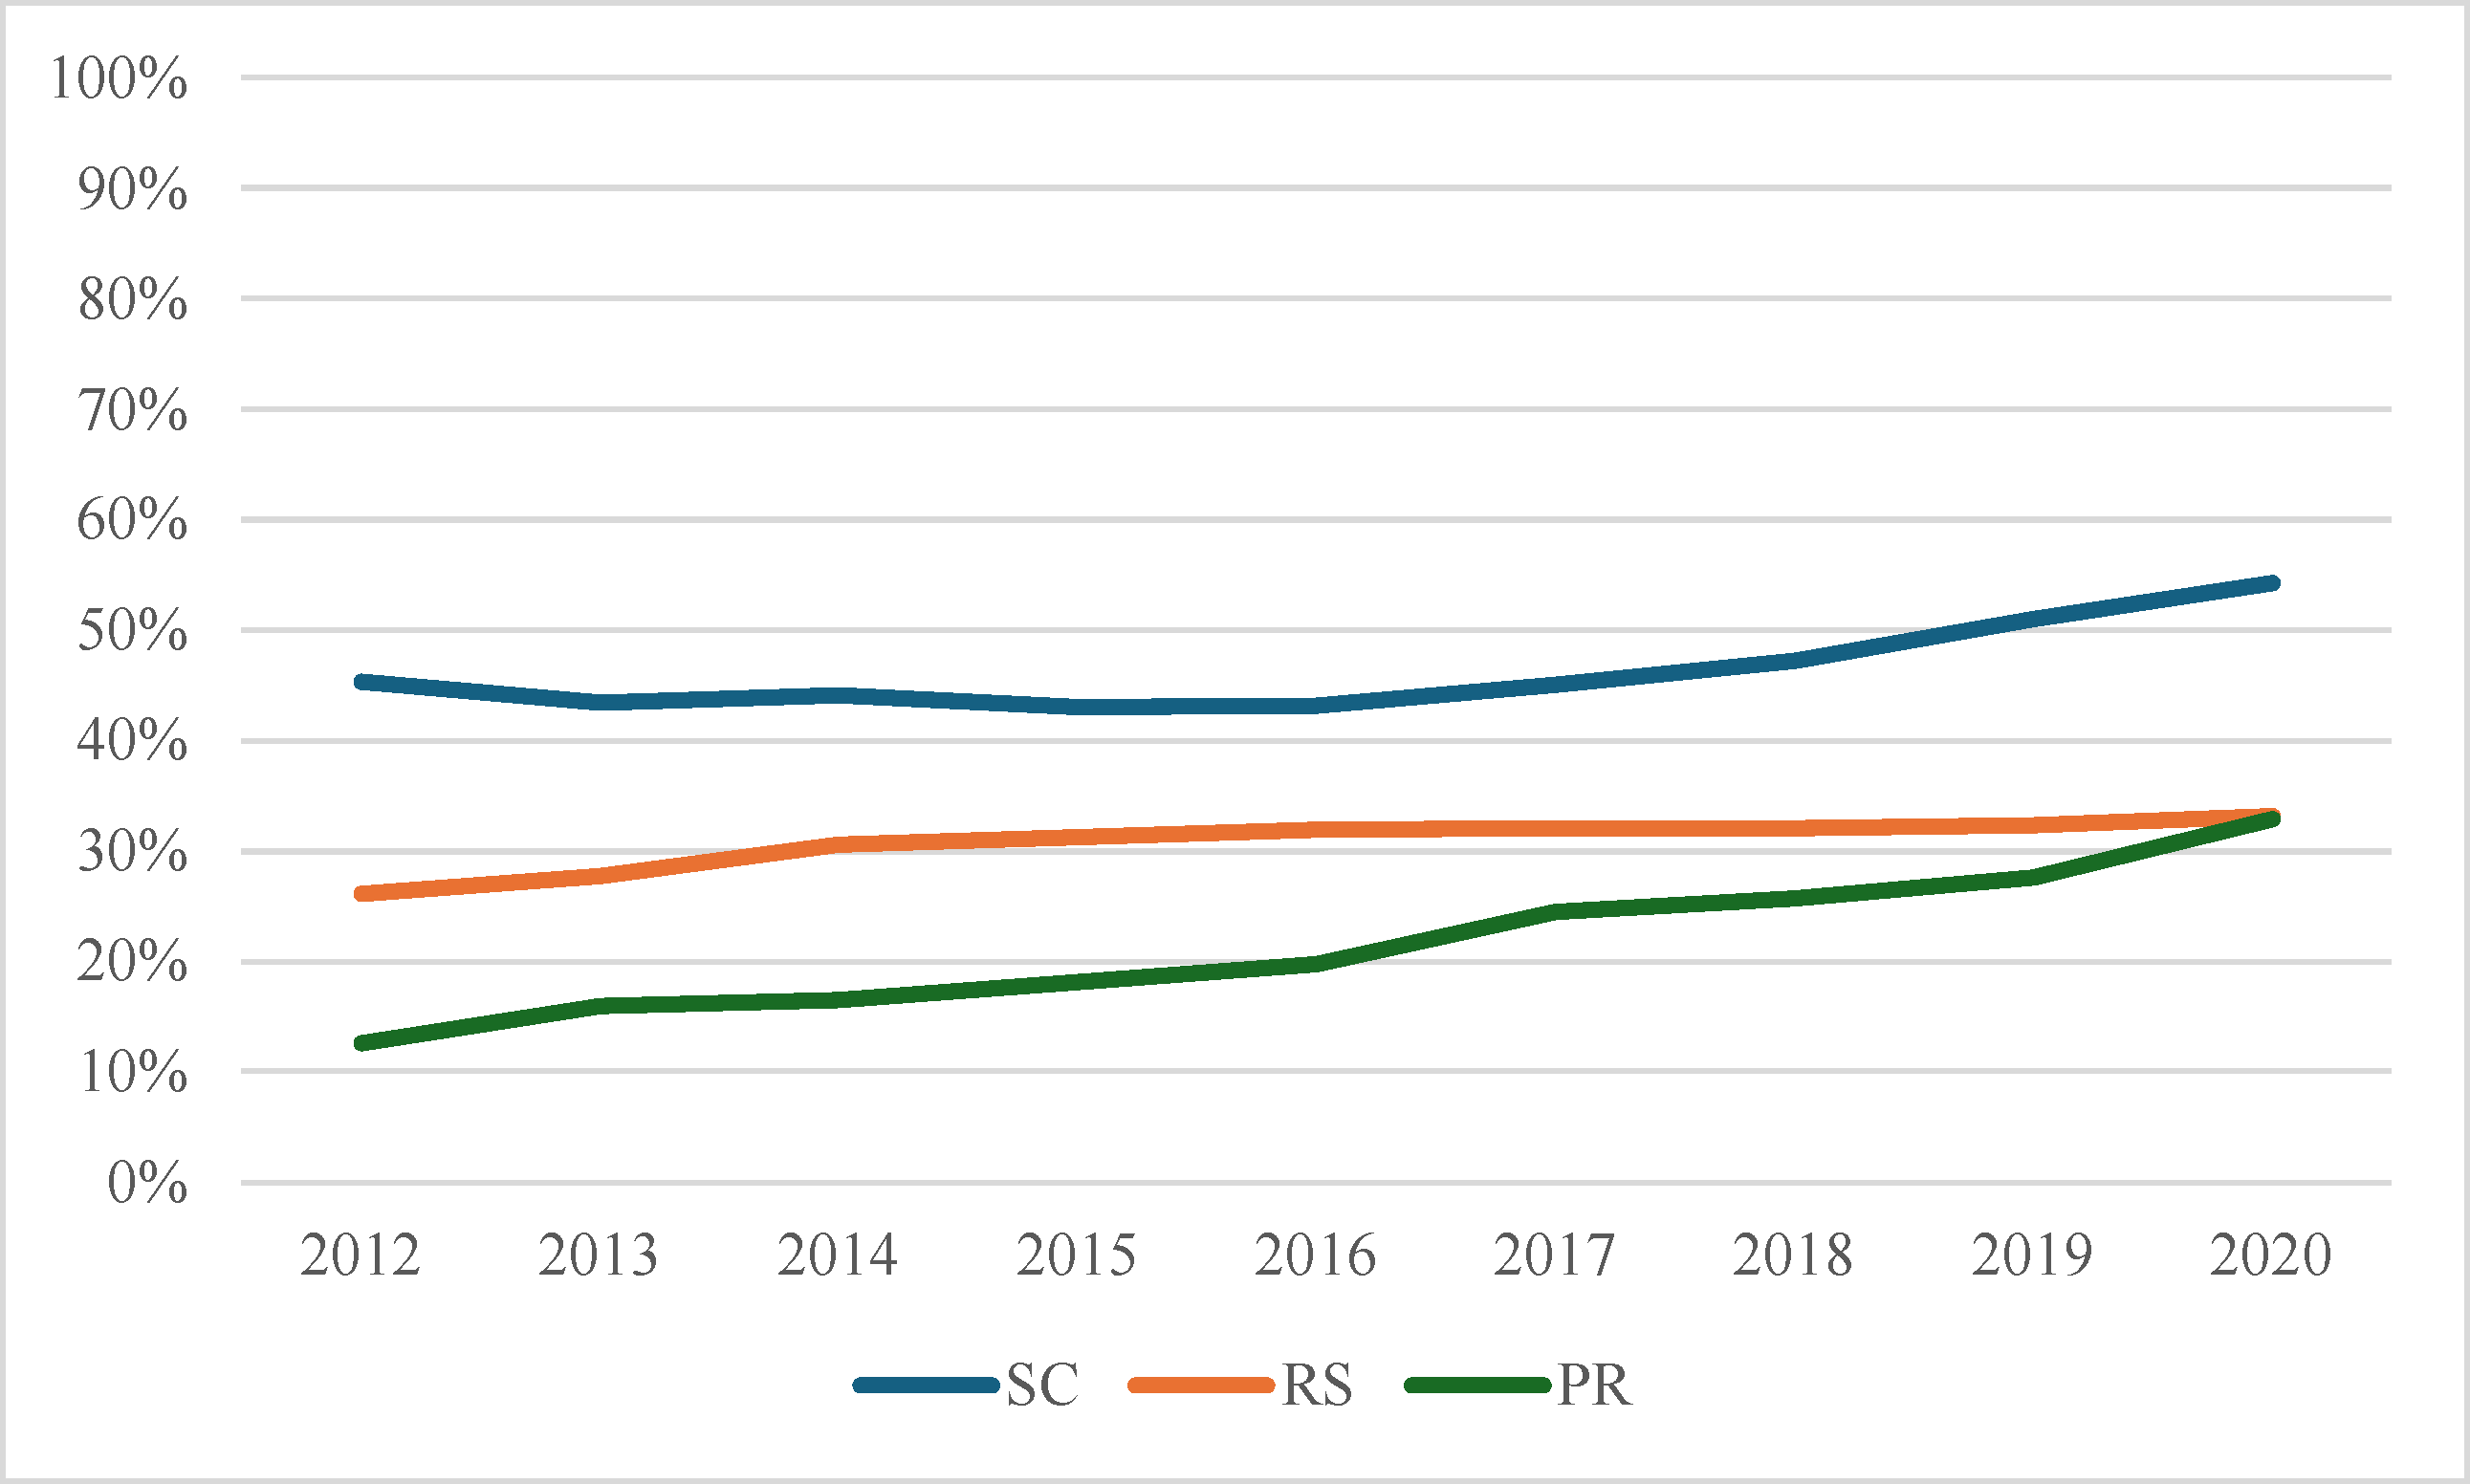
\includegraphics[width=5.0in]{imagens/faltantes-sul.pdf}
    \fonte{Datasus - Sinasc}
    \label{graf:sul}
\end{grafico}

\begin{grafico}
    \centering  
    \caption{Percentual de dados faltantes para a idade do pai ou responsável - Região Norte - 2012-2020}
           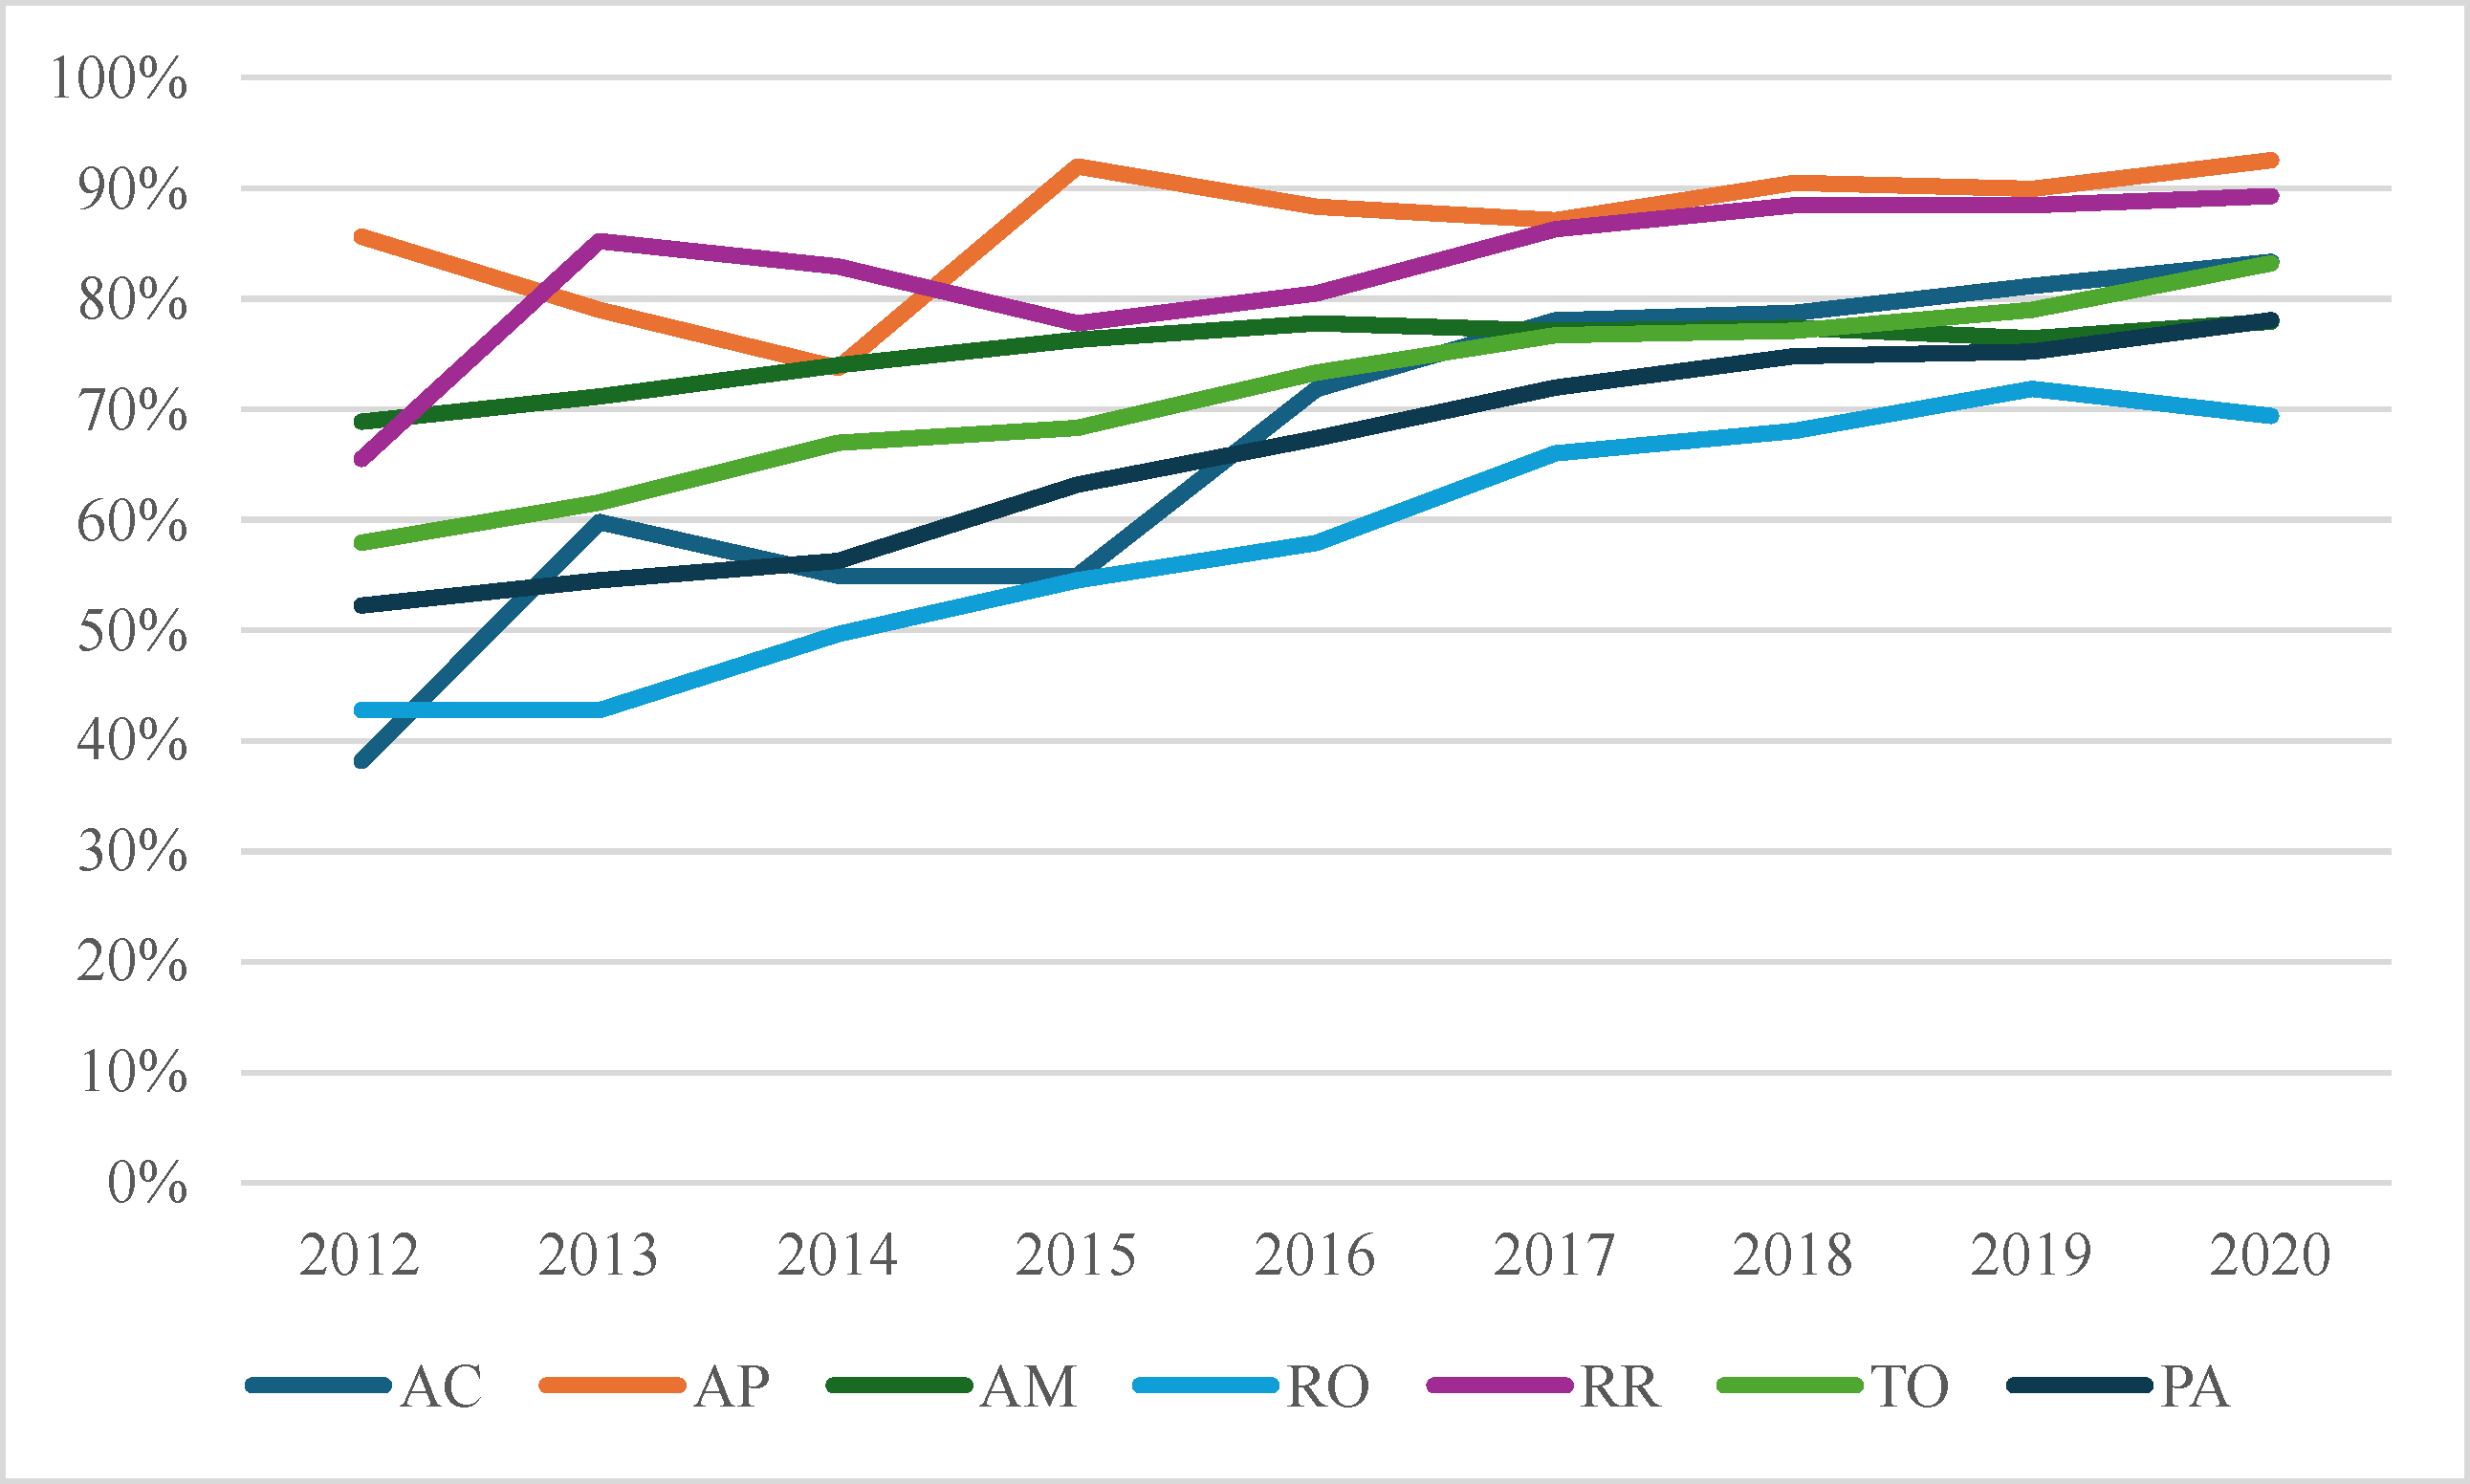
\includegraphics[width=5.0in]{imagens/faltantes-norte.pdf}
    \fonte{Datasus - Sinasc}
    \label{graf:norte}
\end{grafico}

\begin{grafico}
    \centering  
    \caption{Percentual de dados faltantes para a idade do pai ou responsável - Região Centro-Oeste - 2012-2020}
   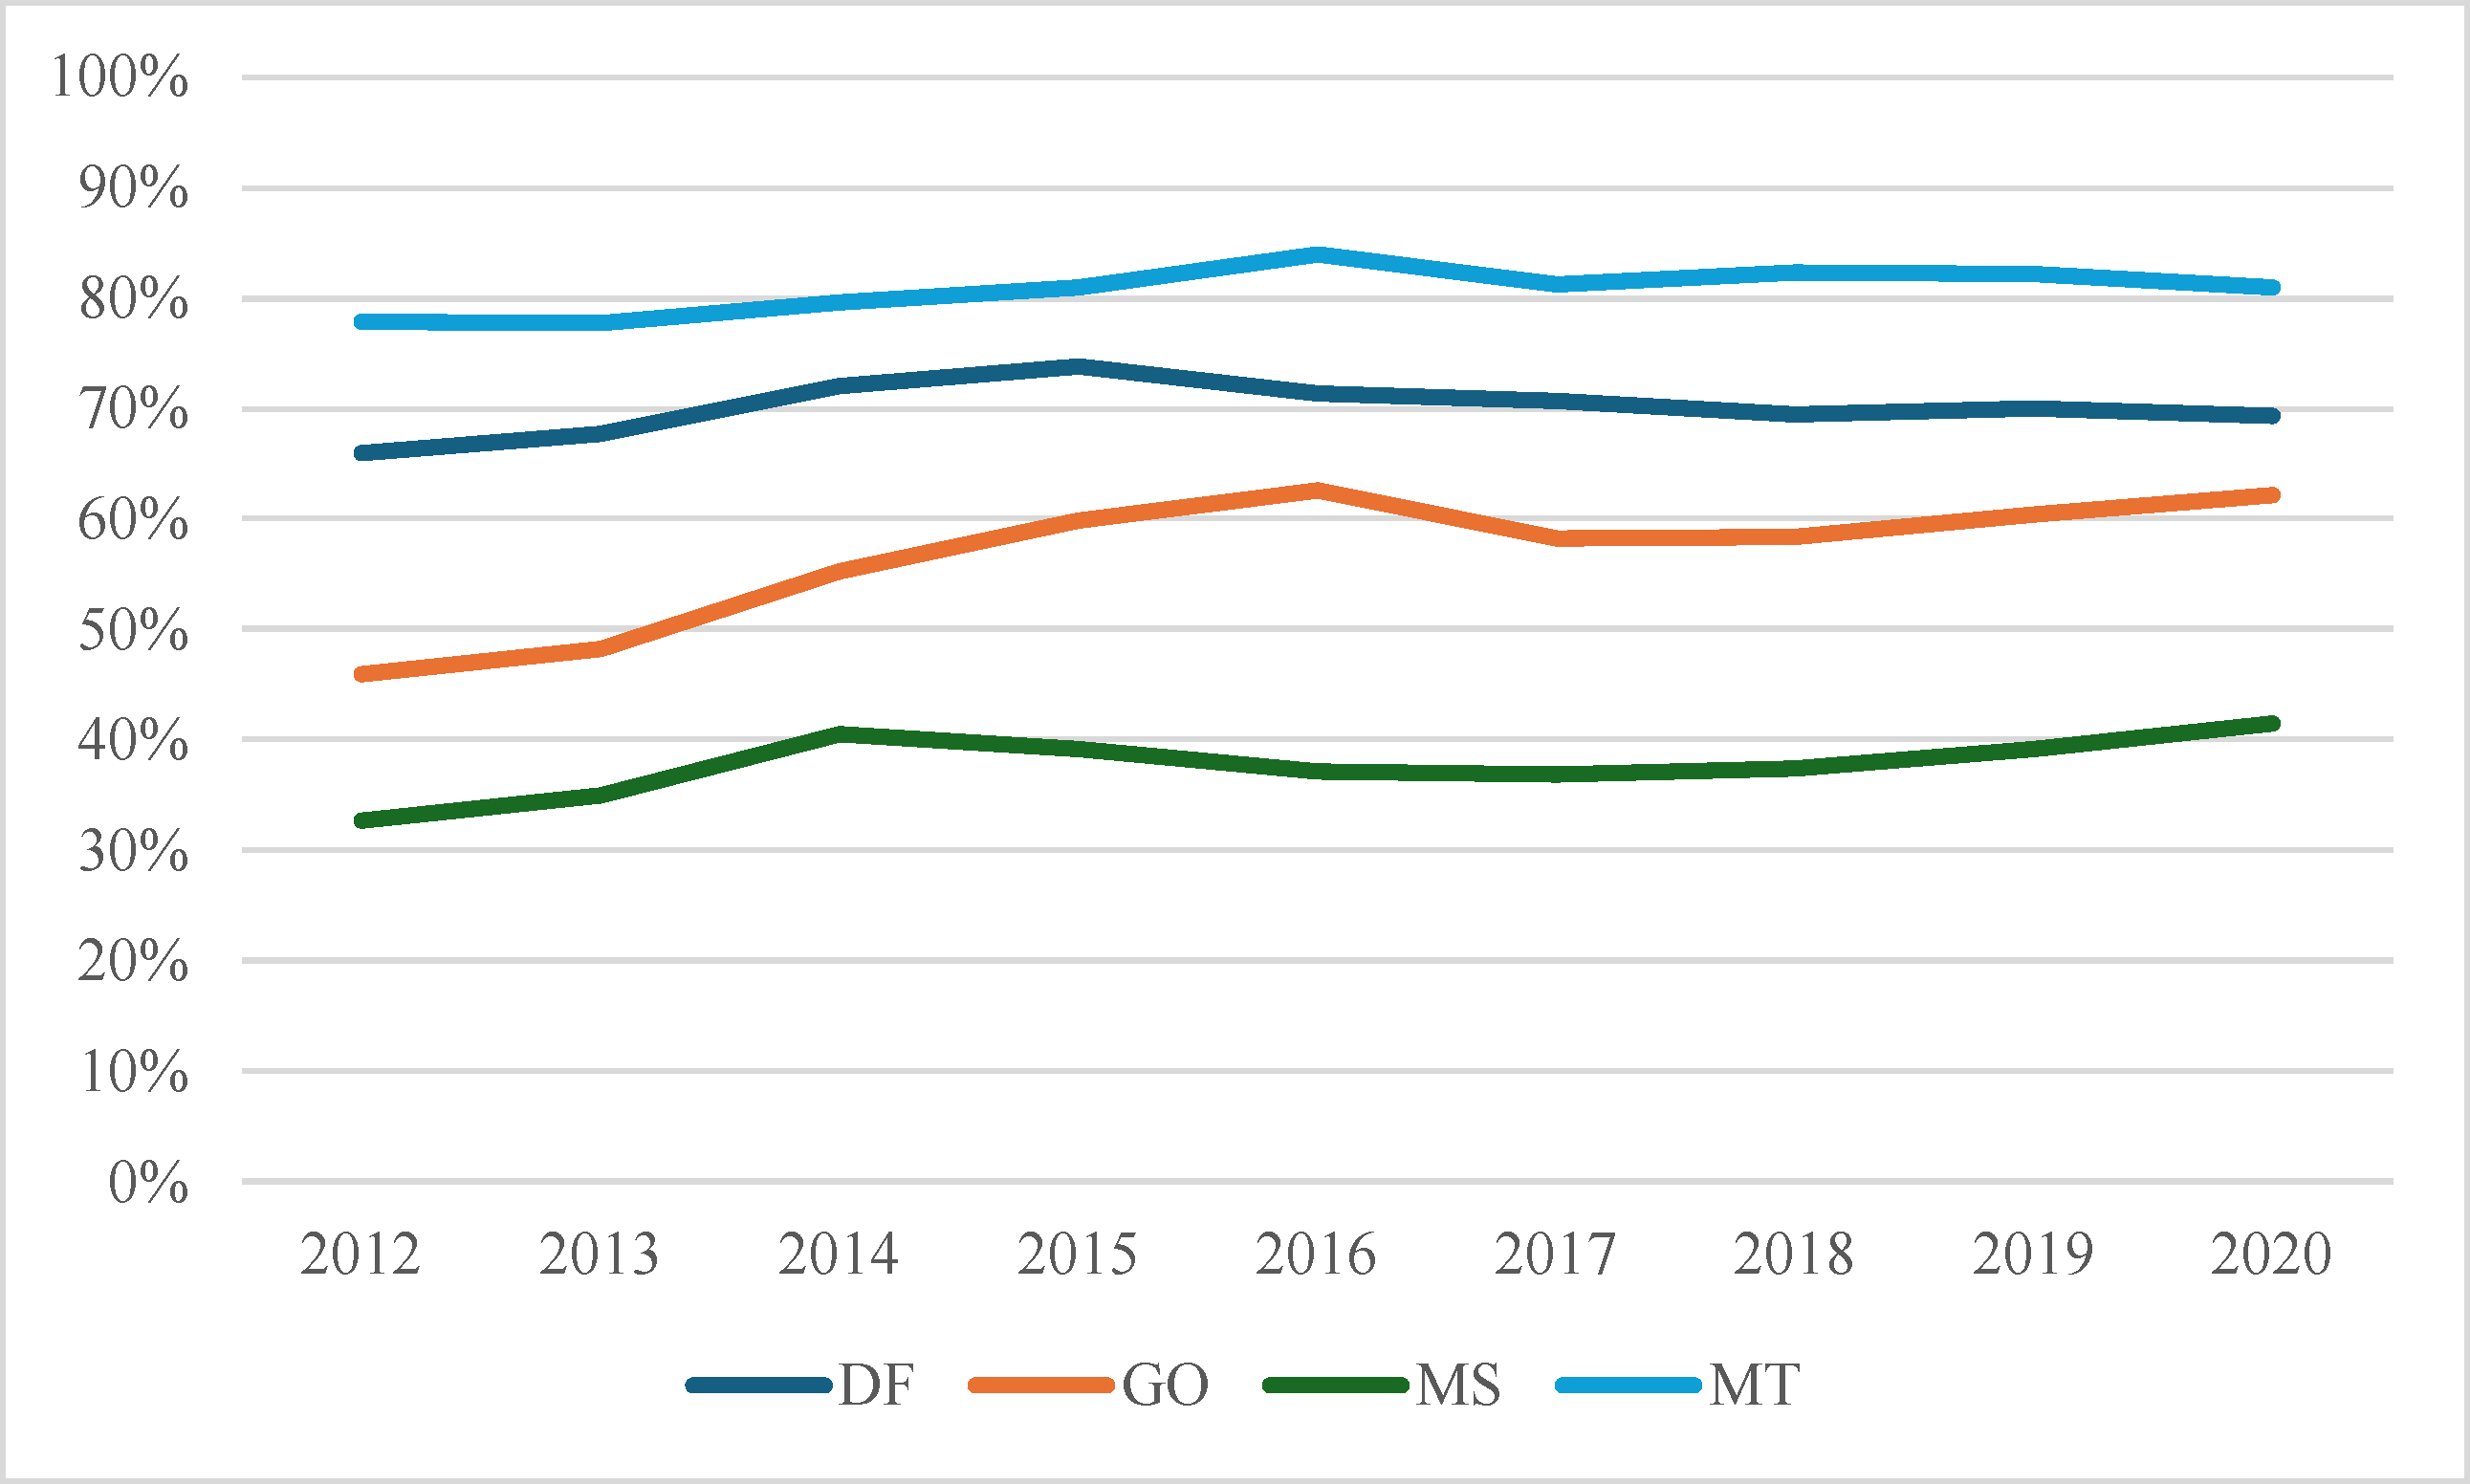
\includegraphics[width=5.0in]{imagens/faltantes-centro-oeste.pdf}
    \fonte{Datasus - Sinasc}
    \label{graf:centro-oeste}
\end{grafico}

\begin{grafico}
    \centering  
    \caption{Percentual de dados faltantes para a idade do pai ou responsável - Região Nordeste - 2012-2020}
        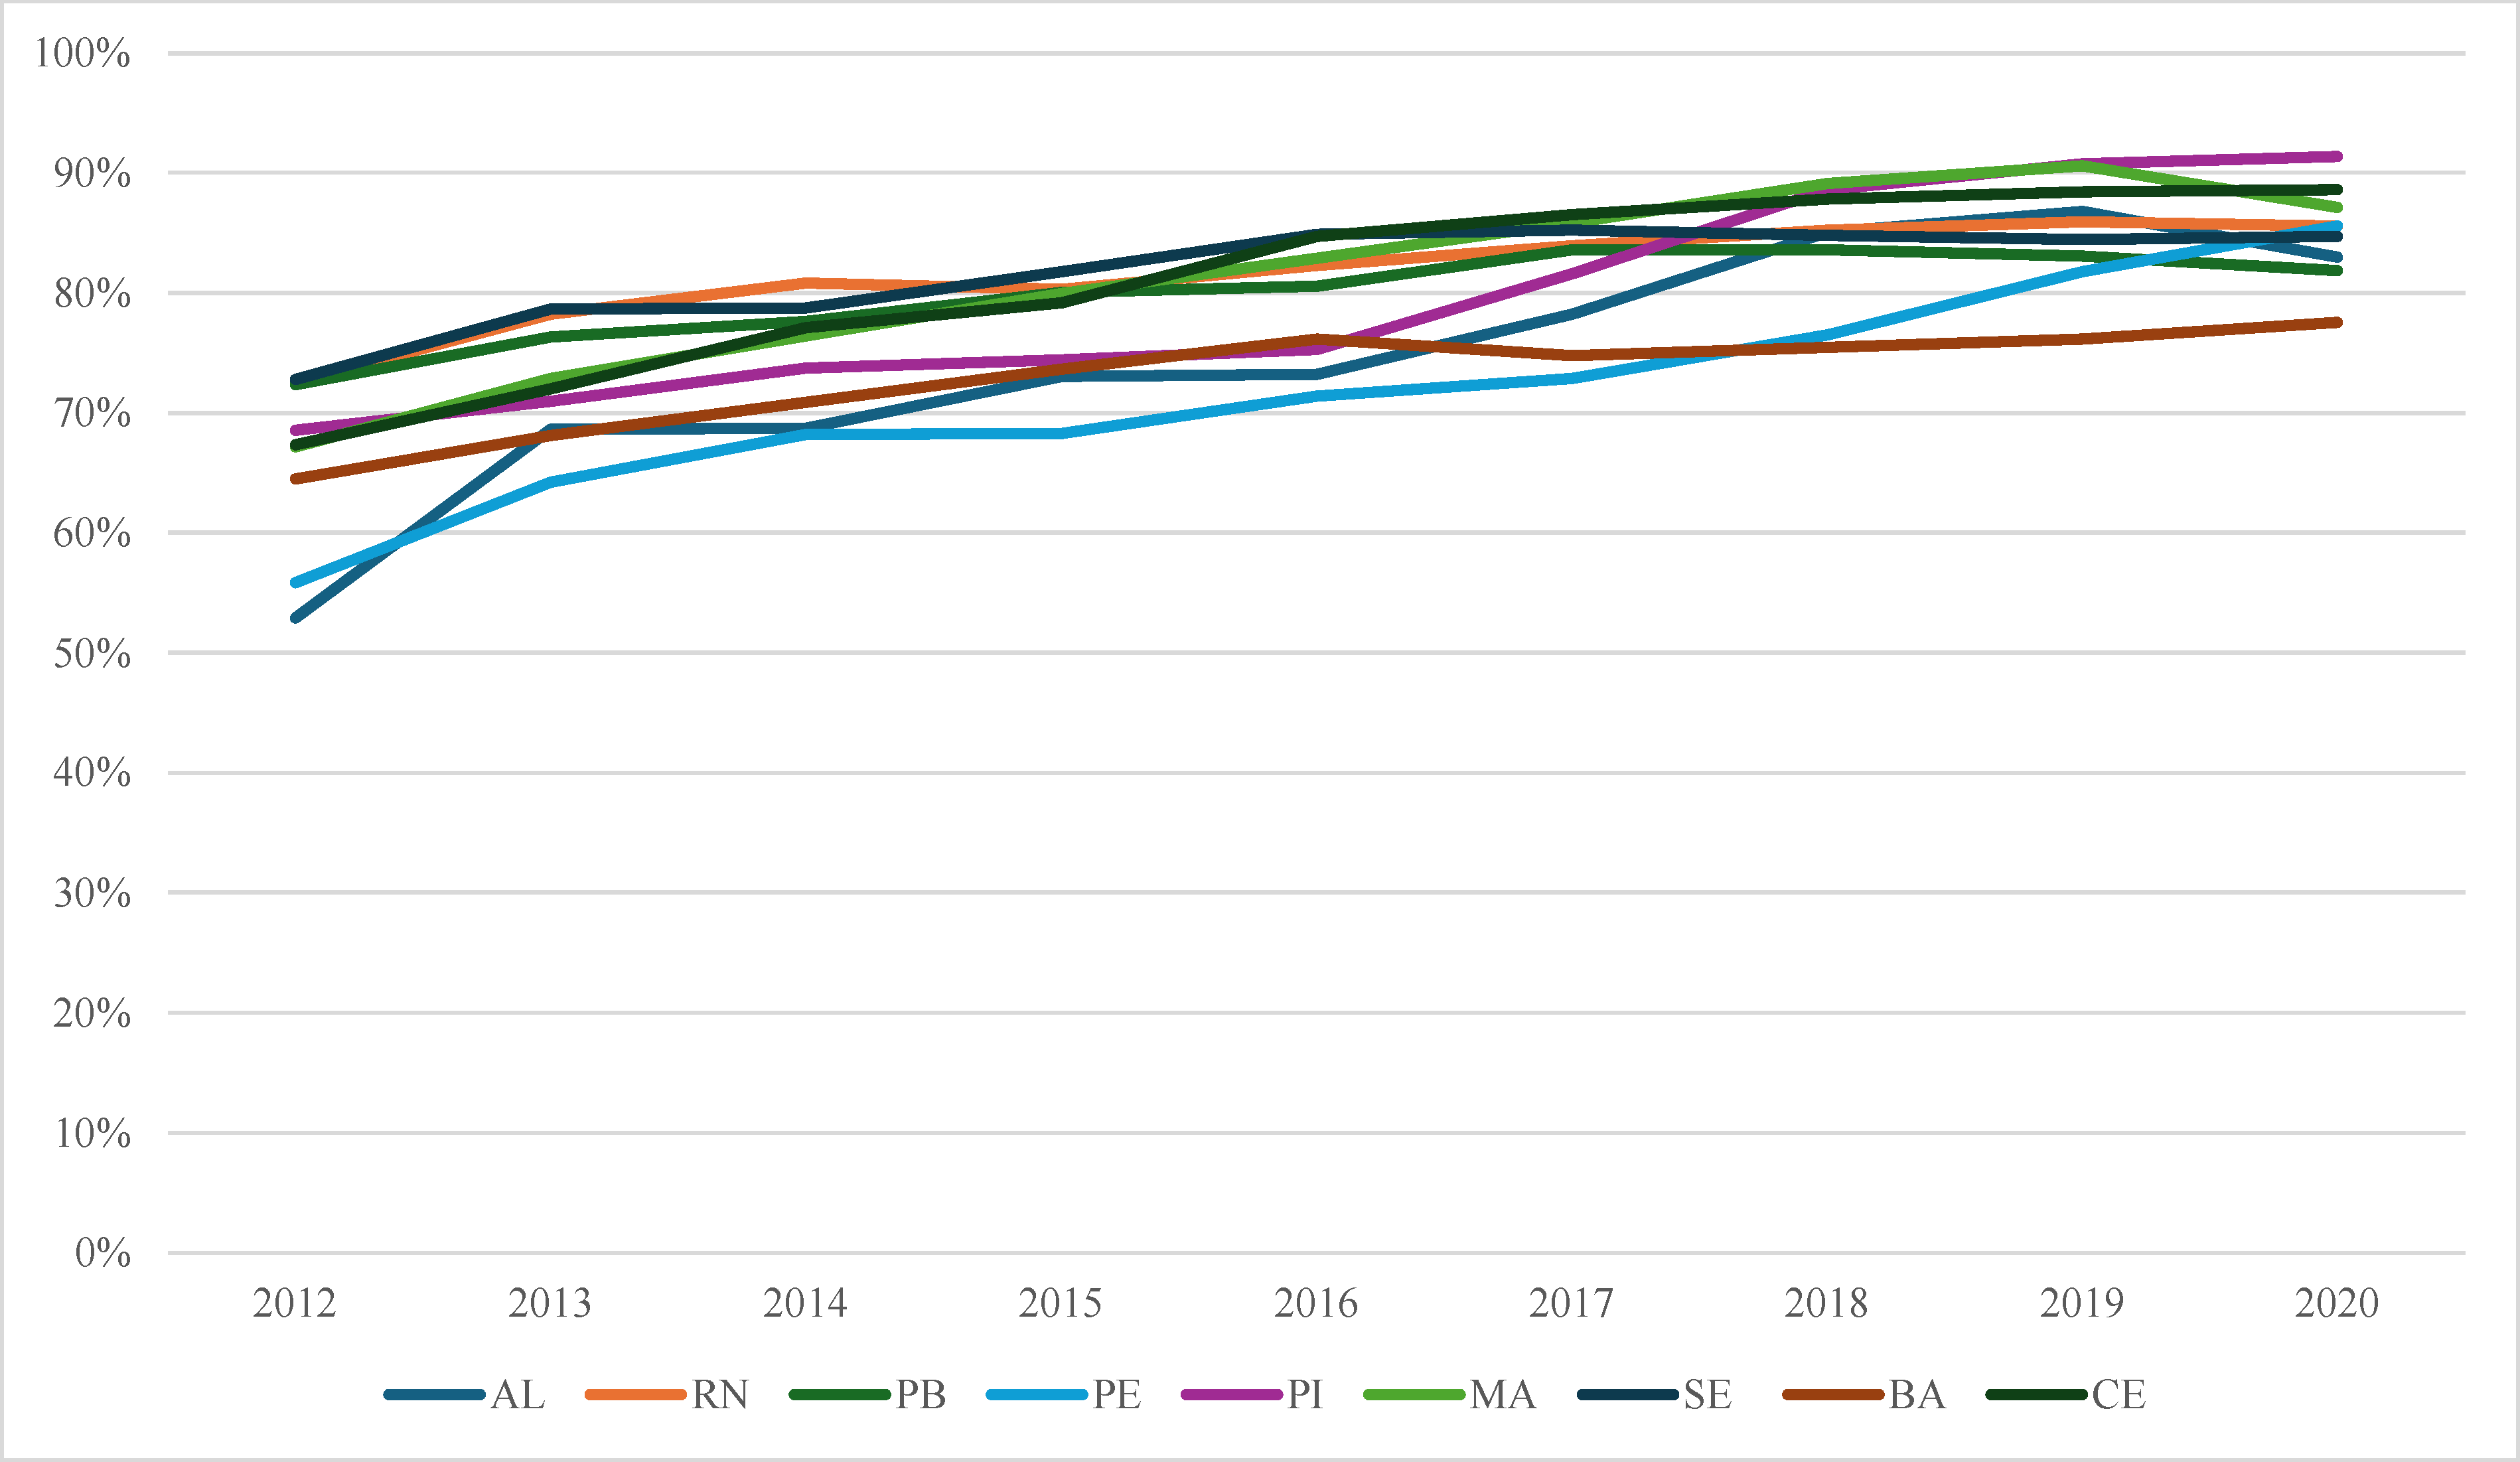
\includegraphics[width=5.0in]{imagens/faltantes-nordeste.pdf}
    \fonte{Datasus - Sinasc}
    \label{graf:nordeste}
\end{grafico}

Na região Norte (\ref{graf:norte}), a proporção de dados faltantes entre as UFs varia de forma menos suavizada através dos anos. Acre e Roraima, por exemplo, apresentam uma diferença de 22\% e 20\% (respectivamente) nos percentuais de dados faltantes de 2012 e 2013. O Amapá apresentou os piores níveis do país em 2012, 2015, 2016, 2017, 2018 e 2020. Em 2020, as UFs apresentaram 93\% de valores não observados, sendo esse o pior cenário entre as UFs no período entre 2012 e 2020.


Os dados da região Centro-Oeste demonstram certa estabilidade nos níveis diferentes de valores faltantes para as UFs. O Mato Grosso apresentou os piores níveis para todos os anos na região, mantendo uma diferença maior que 40\% até 2019 em relação ao Mato Grosso do Sul, a UF com melhores níveis da região. Em 2020 a diferença entre os estados alcança 39\%, a partir de uma suave melhora do Mato Grosso e uma leve piora do Mato Grosso do Sul.

O gráfico \ref{graf:nordeste} demonstra que o Nordeste, enquanto região, apresentou os maiores níveis de valores não observados. Nenhuma das UFs chega a alcançar um nível de pelo menos metade de preenchimento para a variável. Apresentam estabilidade em níveis altos para a proporção de valores faltantes para a idade do pai ou responsável. 





\begin{comment}

          AVALIAR AS RAZÕES PARA O CAMPO SER MARCADO COMO IGNORADO OU SER DEIXADO EM BRANCO ----
        
           FALANDO SOBRE A VARIÁVEL ESCOLARIDADE DA MÃE, MAS ACREDITO QUE O MESMO VALE PARA INFORMAÇÕES SOBRE O PAI: 
        
        A incompletude da escolaridade da mãe foi caracterizada quando o campo da variável no Sinasc apresentava-se em branco ou preenchido como “ignorado”. Todavia,
        
        O campo marcado como ignorado pode estar associado a diferentes fatores. Enquanto em “branco” pode ter relação com o não preenchimento do campo pelo profissional; “ignorado” pode ser pela indisponibilidade de tal informação.
        Nesse ponto de vista, algumas publicações referiram que uma das restrições para a melhor completude da variável foi a ausência das informações no prontuário hospitalar e, para o seu preenchimento, haveria necessidade de uma entrevista com a puérpera ou seu acompanhante, o que, muitas vezes, torna-se difícil por conta de ela não estar em condições de responder ou do seu acompanhante não
        ter conhecimento sobre sua escolaridade, sendo necessária a busca de outras fontes como o cartão da gestante \cite{silvestrin2018avaliaccao}
        %https://www.scielosp.org/pdf/csp/2018.v34n2/e00039217/pt 
\end{comment}


